%-------------------------------------------------------------------------------------------
	\section{Preliminaries}
	\label{sect:preliminaries}
%-------------------------------------------------------------------------------------------

Let $\Sigma$ be a set of types of abstract molecules, or \textit{beads}, and $\Sigma^*$ be the set of finite sequences of beads. 
A bead of type $a \in \Sigma$ is called an $a$-bead. 
Let $w = b_1 b_2\cdots b_n \in \Sigma^*$ be a string of length $n$ for some integer $n$ and bead types $b_1, \ldots, b_n \in \Sigma$.
The \textit{length} of $w$ is denoted by $|w|$, that is, $|w| = n$. 
For two indices $i,j$ with $1\leq i \leq j \leq n$, we let $w[i..j]$ refer to the subsequence $b_i b_{i+1} \cdots b_{j-1} b_{j}$; if $i=j$, then we simplify $w[i..i]$ as $w[i]$.
For $k \ge 1$, $w[1..k]$ is called a \textit{prefix} of $w$. 

Oritatami systems fold their transcript, a sequence of beads, over the triangular grid as suggested in Fig.~\ref{fig:glider} cotranscriptionally based on hydrogen-bond-based interactions (\textit{h-interactions} for short) which their own rule set allow for between adjacent beads of particular types. 
Let $\mathbb{T} = (V, E)$ be the triangular grid graph. 
A directed path $P = p_1 p_2 \cdots p_n$ in $\mathbb{T}$ is a sequence of \textit{pairwise-distinct} points $p_1, p_2, \ldots, p_n \in V$ such that $\{p_i, p_{i+1}\} \in E$ for all $1 \leq i < n$.
Its $i$-th point is referred to as $P[i]$. 
A \textit{rule set} $\mathcal{H} \subseteq \Sigma \times \Sigma$ is a symmetric relation over the set of pairs of bead types. %, that is, for all bead types $a, b \in \Sigma$, $(a, b) \in \mathcal{H}$ implies $(b, a) \in \mathcal{H}$. 
A (finite) \textit{conformation} $C$ is a triple $(P, w, H)$ of a directed path $P$ in $\mathbb{T}$, $w \in \Sigma^*$ of the same length as $P$, and a set of h-interactions $H \subseteq \{\{i,j\} \mid 1 \leq i, i+2 \leq j, \{P[i], P[j]\} \in E\}$.
This is to be interpreted as the sequence $w$ being folded in such a manner that its $i$-th bead $w[i]$ is placed on the $i$-th point $P[i]$ along the path and there is an h-interaction between the $i$-th and $j$-th beads if and only if $(i, j) \in H$. 
The condition $i+2 \leq j$ represents the topological restriction that two consecutive beads along the path cannot h-interact with each other.
%Let $\mathcal{H}$ be a rule set. 
%An h-interaction $(i, j) \in H$ is \textit{valid with respect to $\mathcal{H}$}, or simply \textit{$\mathcal{H}$-valid}, if $(w[i], w[j]) \in \mathcal{H}$. 
%This conformation $C$ is $\mathcal{H}$-valid if all of its h-interactions are $\mathcal{H}$-valid. 
The conformation $C$ is \textit{$\mathcal{H}$-valid} if for all h-interaction $(i, j) \in H$, $(w[i], w[j]) \in \mathcal{H}$. 
For an integer $\alpha \ge 1$, $C$ is \textit{of arity $\alpha$} if the maximum number of h-interactions per bead is $\alpha$, that is, if for any $k \ge 1$, $|\{i \mid (i, k) \in H)\}| + |\{j \mid (k, j) \in H\}| \le \alpha$ and the both sides become equal for some $k$. 
By $\mathcal{C}_{\le \alpha}$, we denote the set of all conformations of arity at most $\alpha$.

Oritatami systems grow conformations by elongating them under their own rule set. 
Given a rule set $\mathcal{H}$ and an $\mathcal{H}$-valid conformation $C_1 = (P, w, H)$, 
we say that another conformation $C_2$ is an \textit{elongation of} $C_1$ \textit{by a bead} $b \in \Sigma$, written as $C_1 \xrightarrow{\mathcal{H}}_b C_2$, if $C_2 = (Pp, wb, H \cup H')$ for some point $p$ not along the path $P$ and set of h-interactions $H' \subseteq \left\{ \{i, |w|+1\} \bigm| 1\leq i < |w|, \{P[i], p\} \in E, (w[i], b) \in \mathcal{H}\right\}$, which can be empty.
Note that $C_2$ is also $\mathcal{H}$-valid.
This operation is recursively extended to the elongation by a finite sequence of beads as: 
for any conformation $C$, $C \xrightarrow{\mathcal{H}}^*_\lambda C$; 
and for a finite sequence of beads $w \in \Sigma^*$ and a bead $b \in \Sigma$,
a conformation $C_1$ is elongated to a conformation $C_2$ by $wb$,
written as $C_1 \xrightarrow{\mathcal{H}}^*_{wb} C_2$, if there is a conformation $C'$ that satisfies
$C_1 \xrightarrow{\mathcal{H}}^*_w C'$ and $C' \xrightarrow{\mathcal{H}}_b C_2$.

A finite \textit{oritatami system} (OS) is a 5-tuple $\Xi = (\mathcal{H}, \alpha, \delta, \sigma,w)$, where 
$\mathcal{H}$ is a rule set,
$\alpha$ is an arity, 
$\delta \geq 1$ is a parameter called the \textit{delay}, 
$\sigma$ is an initial $\mathcal{H}$-valid conformation of arity $\alpha$ called the \textit{seed}, upon which its finite \textit{transcript} $w \in \Sigma^*$ is to be folded by stabilizing beads of $w$ one at a time so as to minimize energy collaboratively with the succeeding $\delta -1$ nascent beads. 
The energy of a conformation $C = (P, w, H)$, denoted by $\Delta G(C)$, is defined to be $-|H|;$ the more h-interactions a conformation has, the more stable it gets.
The set $\mathcal{F}(\Xi)$ of conformations \textit{foldable} by this system is recursively defined as: 
the seed $\sigma$ is in $\mathcal{F}(\Xi)$; and provided that an elongation $C_{i}$ of $\sigma$ by the prefix $w[1..i]$ be foldable (i.e., $C_0 = \sigma$), its further elongation $C_{i+1}$ by the next bead $w[i+1]$ is foldable if
\begin{equation}\label{eq:cotranscriptional_folding}
C_{i+1} \in \argmin_{
\substack{
C \in \mathcal{C}_{\le \alpha} s.t. \\
C_i \xrightarrow{\mathcal{H}}_{w[i+1]}C \\
}
}
\min \left\{ \Delta G(C') \Bigm| 
C \xrightarrow{\mathcal{H}}^*_{w[i+2...i+k]}C', k\le \delta, C' \in \mathcal{C}_{\le \alpha}
\right\}.
\end{equation}
We say that the bead $w[i+1]$ and the h-interactions it forms are \textit{stabilized} according to $C_{i+1}$.
Note that an arity-$\alpha$ OS cannot fold any conformation of arity larger than $\alpha$.
A conformation foldable by $\Xi$ is \textit{terminal} if none of its elongations is foldable by $\Xi$.
The OS $\Xi$ is \textit{deterministic} if for all $i \ge 0$, there exists at most one $C_{i+1}$ that satisfies \eqref{eq:cotranscriptional_folding}. 
%Thus, a deterministic system folds into a unique terminal conformation. 

Let us provide an example of deterministic OS that folds into a motif of great use called the \textit{glider}. 
Let $\Sigma = \{a, a', b, b', \bullet\}$. 
Consider a delay-3 OS whose seed is colored in red in Fig.~\ref{fig:glider}, whose transcript $w$ is a repetition of $a \bullet b' b \bullet a'$, and whose rule set is $\mathcal{H} = \{(a, a'), (b, b')\}$, which makes $\bullet$-beads inert. 

%\begin{figure}[htb]
\begin{wrapfigure}{r}{0.6\linewidth}
\vspace*{-5mm}
\centering
\scalebox{0.4}{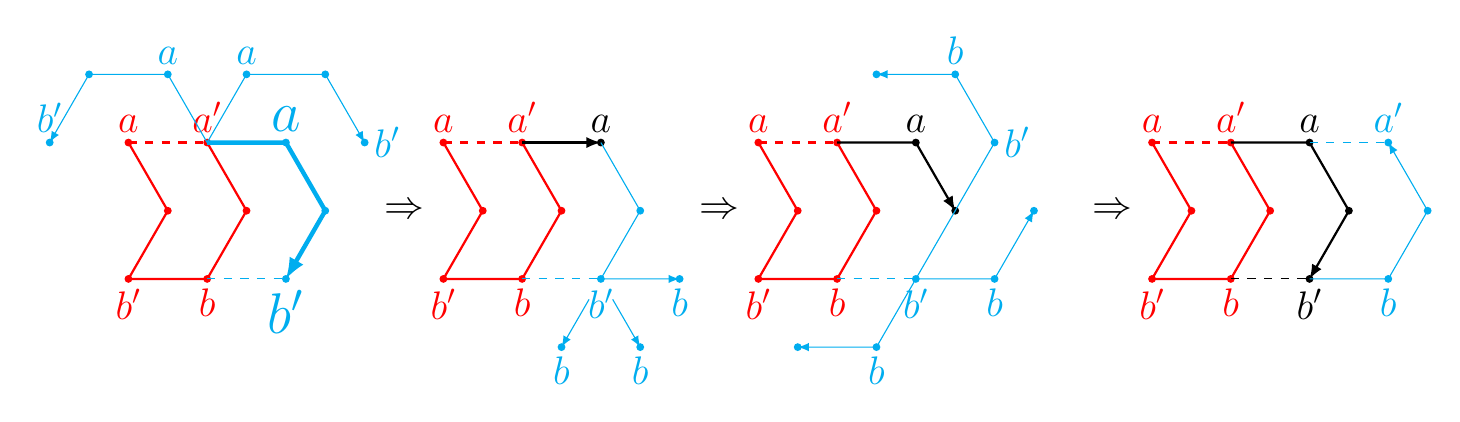
\begin{tikzpicture}
\tikzstyle{mol} = [fill,circle,inner sep=1pt]

\foreach \x in {0, 4, 8, 13} {
\draw[thick, red] (\x, 0) node[mol] {} node[above] {\Large $a$}
-- ++(300:1) node[mol] {} 
-- ++(240:1) node[mol] {} node[below] {\Large $b'$}
-- ++(0:1) node[mol] {} node[below] {\Large $b$}
-- ++(60:1) node[mol] {} 
-- ++(120:1) node[mol] {} node[above] {\Large $a'$}
;
\draw[thick, dashed,red] (\x, 0) -- ++(0:1);
}

\draw[cyan, -latex] (1, 0) -- ++(120:1) node[mol] {} node[above] {\Large $a$} -- ++(180:1) node[mol]{} -- ++(240:1) node[mol] {} node[above] {\Large $b'$};
\draw[cyan, -latex] (1, 0) -- ++(60:1) node[mol] {} node[above] {\Large $a$} -- ++(0:1) node[mol] {} -- ++(300:1) node[mol] {} node[right] {\Large $b'$};
\draw[ultra thick, cyan, -latex] (1, 0) -- ++(0:1) node[mol] {} node[above] {\huge $a$} -- ++(300:1) node[mol] {} -- ++(240:1) node[mol] {} node[below] {\huge $b'$};

\draw[dashed, cyan] (0,0)++(300:2) -- ++(0:1);

\draw (3,0)++(300:1) node {\Large $\Rightarrow$};
\draw (7,0)++(300:1) node {\Large $\Rightarrow$};
\draw (12,0)++(300:1) node {\Large $\Rightarrow$};


\draw[thick, -latex] (5, 0) -- ++(0:1) node[mol] {} node[above] {\Large $a$};

\draw[cyan, -latex] (6, 0) -- ++(300:1) node[mol] {} -- ++(240:1) node[mol] {} node[below] {\Large $b'$} -- ++(0:1) node[mol] {} node[below] {\Large $b$};
\draw[cyan, -latex] (5,0)++(300:2)++(240:0.3) -- ++(240:0.7) node[mol] {} node[below] {\Large $b$};
\draw[cyan, -latex] (5,0)++(300:2.3) -- ++(300:0.7) node[mol] {} node[below] {\Large $b$};
\draw[dashed, cyan] (4,0)++(300:2) -- ++(0:1);


\draw[thick, -latex] (9, 0) -- ++(0:1) node[mol] {} node[above] {\Large $a$}
-- ++(300:1) node[mol] {}
;
\draw[cyan, -latex] (10,0)++(300:1) -- ++(240:1) node[mol] {} node[below] {\Large $b'$}
-- ++(240:1) node[mol] {} node[below] {\Large $b$}
-- ++(180:1) node[mol] {}
;
\draw[cyan, -latex] (9,0)++(300:2) -- ++(0:1) node[mol] {} node[below] {\Large $b$} -- ++(60:1) node[mol] {};
\draw[cyan, -latex] (10,0)++(300:1) -- ++(60:1) node[mol] {} node[right] {\Large $b'$}
-- ++(120:1) node[mol] {} node[above] {\Large $b$}
-- ++(180:1) node[mol] {}
;
\draw[cyan,dashed] (8,0)++(300:2) -- ++(0:1);

\draw[thick, -latex] (14, 0) -- ++(0:1) node[mol] {} node[above] {\Large $a$}
-- ++(300:1) node[mol] {}
-- ++(240:1) node[mol] {} node[below] {\Large $b'$}
;
\draw[dashed] (13,0)++(300:2) -- ++(0:1);
\draw[cyan, -latex] (14,0)++(300:2) -- ++(0:1) node[mol] {} node[below] {\Large $b$}
-- ++(60:1) node[mol] {}
-- ++(120:1) node[mol] {} node[above] {\Large $a'$}
;
\draw[cyan,dashed] (15,0) -- ++(0:1);

\end{tikzpicture}}
\caption{Progression of a glider by distance 1.}
\label{fig:glider}
\vspace*{-3mm}
\end{wrapfigure}
%\end{figure}

%\begin{example}\label{ex:glider}
%A motif called the \emph{glider} explains well how oritatami systems behave. 

By the fragment $w[1..3] = a \bullet b'$, the seed can be elongated in various ways, only three of which are shown in Fig.~\ref{fig:glider} (left). 
The only bead on the fragment capable of a new h-interaction is $b'$ (with a $b$-bead according to $\mathcal{H}$), and for that, the fragment must be folded as bolded in Fig.~\ref{fig:glider} (left). 
The first bead $w[1] = a$ is hence stabilized to the east of the previous bead. 
The next two beads $w[2], w[3]$ are stabilized as illustrated one after another, but we can easily see that the bolded elongation dominates even their stabilization. 
It suffices to observe that neither $w[4]$ nor $w[5]$ can form any new h-interaction. 
When $w[4] = b$ is transcribed (after $w[1]$ is stabilized), $b'$-beads around are either too far or too close. (recall that $w[4]$ cannot interact with $w[3] = b'$). 
In addition, $w[5]$ is inert. 
Thus, they cannot override the bolded ``decision.''
It is easily induced inductively that gliders of arbitrary ``flight distance'' can be folded. 

Gliders also provide a medium to propagate 1-bit at arbitrary distance as the position of their last beads, which is determined by the height (top or bottom) of the first bead and a flying distance.  
%The height (top or bottom) of the first bead determines whether the last bead is stabilized top or bottom after flying a given distance.
For instance, the glider in Fig.~\ref{fig:glider} launches top and thus its last bead (the $a'$) also comes top after traveling the distance 2.
The oritatami system we shall propose exploits this information-carrying capability.
%\end{example}

A \textit{shape} is a set of points on the triangular grid. 
For an integer $c \ge 1$, the \textit{$c$-rhombus scaling} of a shape $S$ is a shape obtained by expanding the distance between the points in $S$ equally by $c$ to obtain another shape $S'$ and replacing each point $\vec{p} \in S'$ by the rhombus whose sides are of length $c$. 
Let $\diamondsuit_c(S)$ be its $c$-rhombus scaling of a shape $S$. 
We say that an OS $\Xi$ \textit{weakly folds} (or ``self-assembles'') $\diamondsuit_c(S)$ if every terminal assembly of $\Xi$ puts its bead only at positions in $\diamondsuit_c(S)$ and it puts at least one bead in all rhombuses of $\diamondsuit_c(S)$. 

